\chapter{Agenten}

\section{Sensoren}

Jeder Agent besitzt 3 Gruppen mit jeweils 4 Sensoren. Alle Sensoren sind visuelle Sensoren mit begrenzter Reichweite und k�nnen nur feststellen, ob sich in ihrem Sichtbereich ein entsprechendes Objekt befindet oder nicht. Andere Objekte blockieren die Sicht, Sichtlinien werden durch einen einfachen Bresenham-Linienalgorithmus bestimmt.\\
Jede Gruppe von Sensoren nimmt einen anderen Typ von Objekt wahr. Die erste Gruppe nimmt das Zielobjekt, die zweite Gruppe andere Agenten und die dritte Gruppe Hindernisse wahr.\\
Ein Sensor ist jeweils in eine bestimmte Richtung ausgerichtet (Norden, Osten, S�den und Westen, wobei auf den Abbildungen Norden immer oben ist) und wird auf ``wahr'' gesetzt, wenn sich in dem von der Sichtweite bestimmten Kegel ein entsprechendes Objekt befindet.\\
In Abbildung ~\ref{sight_directions:fig} sind alle Sichtkegel (dunkler und heller Bereich) und �berwachungsreichweiten (heller Bereich) f�r die einzelnen Richtungen dargestellt. Als Sandardwerte wird hier eine Sichtweite von \(5.0\) und eine �berwachungsreichweite von \(3.0\) verwendet, der �berwachte Bereich ist also eine Teilmenge des sichtbaren Bereichs.

\begin{figure}[htbp]
\centerline{	
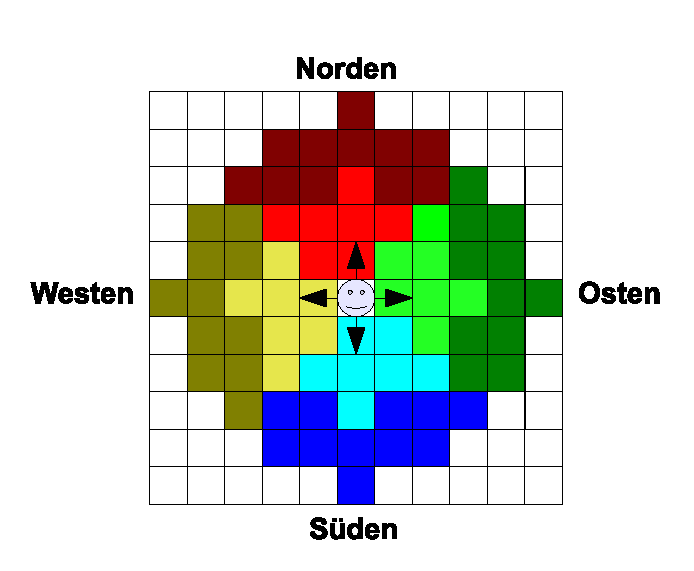
\includegraphics{sight_directions.eps}
}
\caption[Sichtkegel und �berwachungsreichweite eines Agenten]{Sichtkegel und �berwachungsreichweite eines Agenten, jeweils f�r die einzelnen Richtungen}
\label{sight_directions:fig}
\end{figure}

\section{F�higkeiten}

Jeder Agent kann in jedem Schritt zwischen 5 verschiedenen Aktionen w�hlen, die den vier Richtungen plus einer Aktion, bei der der Agent sich nicht bewegt, entsprechen. Agenten k�nnen pro Zeiteinheit genau einen Schritt durchf�hren. Das Zielobjekt kann je nach Szenarioparameter mehrere Schritte ausf�hren.

\section{Ablauf der Bewegung}
Alle Agenten werden nacheinander in der Art abgearbeitet, dass der jeweilige Agent die aktuellen Sensordaten aus der Umgebung holt und anhand dieser die n�chste Aktion bestimmt. Ung�ltige Aktionen, d.h. der Versuch sich auf ein besetztes Feld zu bewegen, schlagen fehl und der Agent f�hrt in diesem Schritt keine Aktion aus, wird aber nicht weiter bestraft. Eine detaillierte Beschreibung wird in Kapitel~\ref{conclusion:cha} geliefert.

\section{Grunds�tzliche Algorithmen der Agenten}

Neben denjenigen Algorithmen, die auf LCS basieren und in Kapitel~\ref{lcs:cha} besprochen werden, gibt es folgende Grundtypen, die dazu dienen, die Qualit�t der anderen Algorithmen einzuordnen. Wesentliches Merkmal im Vergleich zu auf LCS basierenden Algorithmen ist, dass sie statische, handgeschriebene Regeln benutzen und den Erfolg oder Misserfolg ihrer Aktionen ignorieren, d.h. ihre Regeln nicht anpassen.

\subsection{``Randomized''}\label{randomized_movement:sec}
In jedem Schritt wird eine zuf�llige Aktion ausgef�hrt. Abbildung ~(\ref{agent_random:fig}) zeigt eine Beispielsituation bei der der Agent jegliche Sensordaten ignoriert und eine Aktion zuf�llig ausw�hlen wird.

\begin{figure}[htbp]
\centerline{	
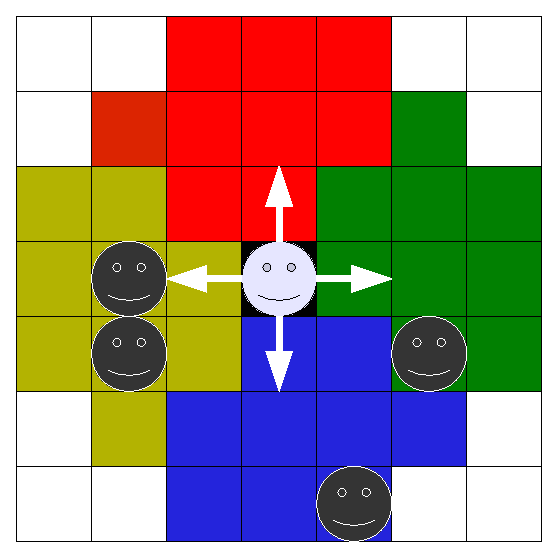
\includegraphics{agent_random.eps}
}
\caption[Sich zuf�llig bewegender Agent]{Agent bewegt sich in eine zuf�llige Richtung (oder bleibt stehen)}
\label{agent_random:fig}
\end{figure}

\subsection{``Simple AI Agent''}
Ist das Zielobjekt in Sichtweite, bewegt sich dieser Agent auf das Ziel zu. Ist es nicht in Sichtweite, f�hrt er eine zuf�llige Aktion aus. Abbildung ~(\ref{simple_agent_to_goal:fig}) zeigt eine Beispielsituation bei der sich das Zielobjekt (Stern) im S�den befindet, der Agent die anderen Agenten ignoriert und sich auf das Ziel zubewegen m�chte. 

\begin{figure}[htbp]
\centerline{	
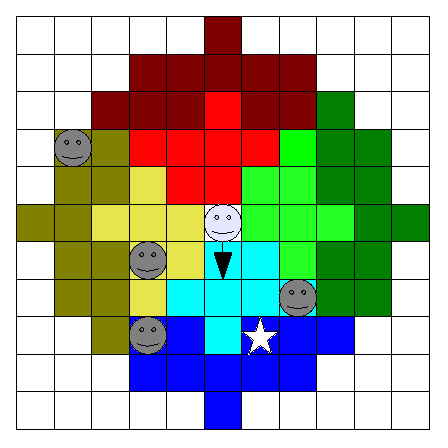
\includegraphics{simple_agent_to_goal.eps}
}
\caption[Einfacher Agent]{Einfacher Agent : Sofern es sichtbar ist bewegt sich der Agent auf das Zielobjekt zu}
\label{simple_agent_to_goal:fig}
\end{figure}

\subsection{``Intelligent AI Agent''}
Ist der Zielobjekt in Sicht, verh�lt sich dieser Algorithmus wie ``Simple AI Agent''. Ist das Zielobjekt dagegen nicht in Sicht, wird versucht, anderen Agenten auszuweichen, um ein m�glichst breit gestreutes Netz aus Agenten aufzubauen. In der Implementation hei�t das, dass unter allen Richtungen, in denen kein anderer Agent gesichtet wurde, eine Richtung zuf�llig ausgew�hlt wird. Falls alle Richtungen belegt (oder alle frei) sind, wird aus allen Richtungen eine zuf�llig ausgew�hlt wird. In Abbildung ~(\ref{intelligent_agent:fig}) sieht der Agent das Zielobjekt nicht und w�hlt deswegen eine Richtung, in der der Sensor keine Agenten anzeigt, in diesem Fall Norden.

\begin{figure}[htbp]
\centerline{	
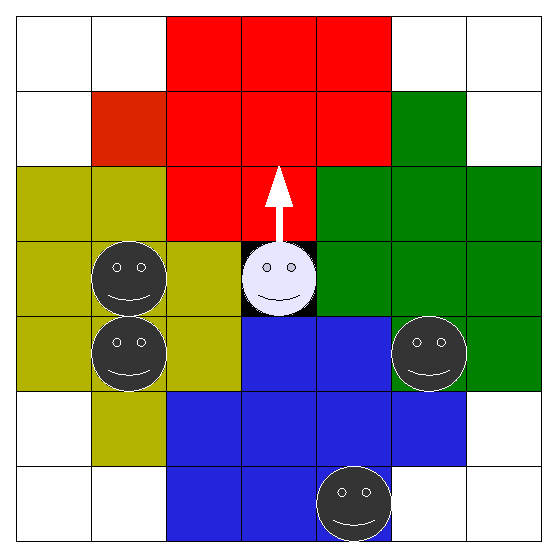
\includegraphics{intelligent_agent.eps}
}
\caption[Sich intelligent verhaltender Agent]{Intelligenter Agent : Falls das Zielobjekt nicht sichtbar ist bewegt sich der Agent von anderen Agenten weg}
\label{intelligent_agent:fig}
\end{figure}
